\chapter[QR Factorization and Householder Reflections]{QR Factorization and Householder Reflections:\\Geometry, Numerical Stability, and Algorithms}
\label{chap:qr-factorization-householder-reflections}
\label{chap:fattorizzazione-qr-riflessioni-householder-en}

This chapter introduces and constructively analyzes the \textbf{QR Factorization}, one of the cornerstones of modern numerical linear algebra for scientific computing, overdetermined linear systems (least squares problems), and spectral eigenvalue computation~\cite{golub2013matrix,trefethen1997numerical}. After formalizing the general existence theorem and the geometric distinction between the full decomposition (\textit{Full QR}) and the economical variant (\textit{Thin QR}), we introduce the family of \textbf{Householder reflectors} (elementary rank-1 orthogonal transformations). We prove the fundamental reflection lemma and address the critical impact of finite-precision floating-point arithmetic (catastrophic cancellation) in selecting the numerically stable reflector. The discussion proceeds with the algorithmic formulation of the factorization via sequences of reflections, asymptotic complexity analysis, the conditional uniqueness theorem, and a comprehensive, fully worked $3 \times 3$ numerical example.

\FloatBarrier
\section{Introduction to QR Factorization and Matrix Forms}
\label{sec:intro-qr-forms-en}

\subsection{Existence Theorem for QR Factorization}

\begin{theorem}[Full QR Factorization]
\label{thm:qr-existence-full-en}
For every real rectangular matrix $A \in \R^{m \times n}$, there exist:
\begin{enumerate}
    \item a square orthogonal matrix $Q \in \R^{m \times m}$, such that:
    \begin{equation}
        Q^T Q = Q Q^T = I_m;
    \end{equation}
    \item an extended upper triangular matrix $R \in \R^{m \times n}$, such that:
    \begin{equation}
        R_{i,j} = 0 \quad \text{for all } i > j;
    \end{equation}
\end{enumerate}
such that their product exactly reconstructs the initial matrix:
\begin{equation}
    A = Q R.
\end{equation}
\end{theorem}

The computational significance of Theorem~\ref{thm:qr-existence-full-en} lies in the optimal conditioning of orthogonal matrices: since $\|Q\|_2 = 1$ and $\cond_2(Q) = 1$, matrix multiplication by $Q$ does not amplify rounding errors, perfectly preserving Euclidean norms and data energy.

\subsection[Geometry and Dimensions in the Three Cases]{Geometry and Dimensions in the Three Cases}
Depending on the dimensional ratio between the number of rows $m$ and columns $n$, the factorization takes distinct structural shapes:

\begin{figure}[H]
\centering
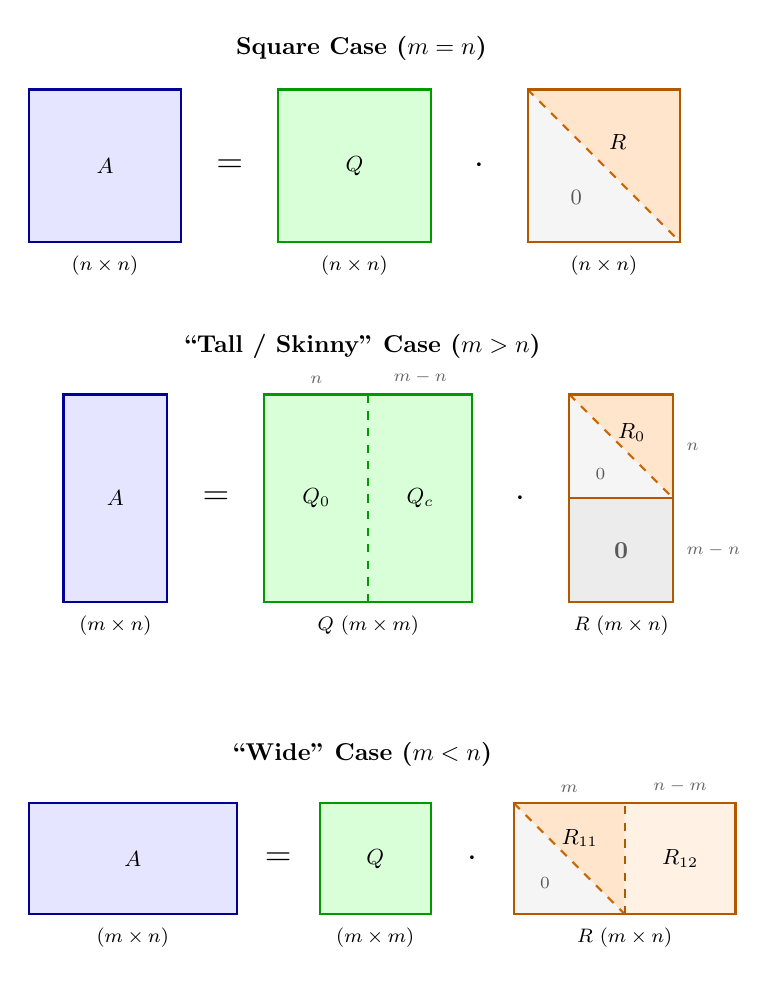
\begin{tikzpicture}[scale=0.88, every node/.style={transform shape}]
    % =========================================================
    % CASE 1: SQUARE (m = n)
    % =========================================================
    \begin{scope}[yshift=0cm]
        \node[font=\bfseries] at (5.0, 2.8) {Square Case ($m = n$)};
        
        % Matrix A (n x n)
        \draw[thick, fill=blue!10, draw=blue!60!black] (0.2, 0) rectangle (2.4, 2.2);
        \node[font=\small\bfseries] at (1.3, 1.1) {$A$};
        \node[below=2pt, font=\footnotesize] at (1.3, 0) {$(n \times n)$};
        
        % Equals sign
        \node[font=\Large\bfseries] at (3.1, 1.1) {$=$};
        
        % Matrix Q (n x n)
        \draw[thick, fill=green!15, draw=green!60!black] (3.8, 0) rectangle (6.0, 2.2);
        \node[font=\small\bfseries] at (4.9, 1.1) {$Q$};
        \node[below=2pt, font=\footnotesize] at (4.9, 0) {$(n \times n)$};
        
        % Dot sign
        \node[font=\Large\bfseries] at (6.7, 1.1) {$\cdot$};
        
        % Matrix R (n x n)
        \fill[orange!20] (7.4, 2.2) -- (9.6, 2.2) -- (9.6, 0) -- cycle;
        \fill[gray!8] (7.4, 2.2) -- (7.4, 0) -- (9.6, 0) -- cycle;
        \draw[thick, dashed, draw=orange!80!black] (7.4, 2.2) -- (9.6, 0);
        \draw[thick, draw=orange!70!black] (7.4, 0) rectangle (9.6, 2.2);
        \node[font=\small\bfseries] at (8.7, 1.45) {$R$};
        \node[font=\small, text=gray!70!black] at (8.1, 0.65) {$0$};
        \node[below=2pt, font=\footnotesize] at (8.5, 0) {$(n \times n)$};
    \end{scope}

    % =========================================================
    % CASE 2: TALL / SKINNY (m > n)
    % =========================================================
    \begin{scope}[yshift=-5.2cm]
        \node[font=\bfseries] at (5.0, 3.7) {``Tall / Skinny'' Case ($m > n$)};
        
        % Matrix A (m x n)
        \draw[thick, fill=blue!10, draw=blue!60!black] (0.7, 0) rectangle (2.2, 3.0);
        \node[font=\small\bfseries] at (1.45, 1.5) {$A$};
        \node[below=2pt, font=\footnotesize] at (1.45, 0) {$(m \times n)$};
        
        % Equals sign
        \node[font=\Large\bfseries] at (2.9, 1.5) {$=$};
        
        % Matrix Q (m x m)
        \draw[thick, fill=green!15, draw=green!60!black] (3.6, 0) rectangle (6.6, 3.0);
        \draw[thick, dashed, draw=green!60!black] (5.1, 0) -- (5.1, 3.0);
        \node[font=\small\bfseries] at (4.35, 1.5) {$Q_0$};
        \node[font=\small\bfseries] at (5.85, 1.5) {$Q_c$};
        \node[above=1pt, font=\scriptsize, text=gray!80!black] at (4.35, 3.0) {$n$};
        \node[above=1pt, font=\scriptsize, text=gray!80!black] at (5.85, 3.0) {$m-n$};
        \node[below=2pt, font=\footnotesize] at (5.1, 0) {$Q \ (m \times m)$};
        
        % Dot sign
        \node[font=\Large\bfseries] at (7.3, 1.5) {$\cdot$};
        
        % Matrix R (m x n)
        % Block R_0 (n x n upper triangular)
        \fill[orange!20] (8.0, 3.0) -- (9.5, 3.0) -- (9.5, 1.5) -- cycle;
        \fill[gray!8] (8.0, 3.0) -- (8.0, 1.5) -- (9.5, 1.5) -- cycle;
        \draw[thick, dashed, draw=orange!80!black] (8.0, 3.0) -- (9.5, 1.5);
        \node[font=\small\bfseries] at (8.9, 2.45) {$R_0$};
        \node[font=\scriptsize, text=gray!70!black] at (8.45, 1.85) {$0$};
        % Block 0 lower ((m-n) x n)
        \fill[gray!15] (8.0, 0) rectangle (9.5, 1.5);
        \node[font=\bfseries, text=gray!70!black] at (8.75, 0.75) {$\mathbf{0}$};
        % Borders and dividers
        \draw[thick, draw=orange!70!black] (8.0, 1.5) -- (9.5, 1.5);
        \draw[thick, draw=orange!70!black] (8.0, 0) rectangle (9.5, 3.0);
        \node[right=2pt, font=\scriptsize, text=gray!80!black] at (9.5, 2.25) {$n$};
        \node[right=2pt, font=\scriptsize, text=gray!80!black] at (9.5, 0.75) {$m-n$};
        \node[below=2pt, font=\footnotesize] at (8.75, 0) {$R \ (m \times n)$};
    \end{scope}

    % =========================================================
    % CASE 3: WIDE (m < n)
    % =========================================================
    \begin{scope}[yshift=-9.7cm]
        \node[font=\bfseries] at (5.0, 2.3) {``Wide'' Case ($m < n$)};
        
        % Matrix A (m x n)
        \draw[thick, fill=blue!10, draw=blue!60!black] (0.2, 0) rectangle (3.2, 1.6);
        \node[font=\small\bfseries] at (1.7, 0.8) {$A$};
        \node[below=2pt, font=\footnotesize] at (1.7, 0) {$(m \times n)$};
        
        % Equals sign
        \node[font=\Large\bfseries] at (3.8, 0.8) {$=$};
        
        % Matrix Q (m x m)
        \draw[thick, fill=green!15, draw=green!60!black] (4.4, 0) rectangle (6.0, 1.6);
        \node[font=\small\bfseries] at (5.2, 0.8) {$Q$};
        \node[below=2pt, font=\footnotesize] at (5.2, 0) {$(m \times m)$};
        
        % Dot sign
        \node[font=\Large\bfseries] at (6.6, 0.8) {$\cdot$};
        
        % Matrix R (m x n)
        % Block R_11 (m x m upper triangular)
        \fill[orange!20] (7.2, 1.6) -- (8.8, 1.6) -- (8.8, 0) -- cycle;
        \fill[gray!8] (7.2, 1.6) -- (7.2, 0) -- (8.8, 0) -- cycle;
        \draw[thick, dashed, draw=orange!80!black] (7.2, 1.6) -- (8.8, 0);
        \node[font=\small\bfseries] at (8.15, 1.1) {$R_{11}$};
        \node[font=\scriptsize, text=gray!70!black] at (7.65, 0.45) {$0$};
        % Block R_12 (m x (n-m) dense)
        \fill[orange!10] (8.8, 0) rectangle (10.4, 1.6);
        \node[font=\small\bfseries] at (9.6, 0.8) {$R_{12}$};
        % Borders and dividers
        \draw[thick, dashed, draw=orange!70!black] (8.8, 0) -- (8.8, 1.6);
        \draw[thick, draw=orange!70!black] (7.2, 0) rectangle (10.4, 1.6);
        \node[above=1pt, font=\scriptsize, text=gray!80!black] at (8.0, 1.6) {$m$};
        \node[above=1pt, font=\scriptsize, text=gray!80!black] at (9.6, 1.6) {$n-m$};
        \node[below=2pt, font=\footnotesize] at (8.8, 0) {$R \ (m \times n)$};
    \end{scope}
\end{tikzpicture}
\caption{Dimensional structure of the QR decomposition across the three geometric regimes ($m = n$, $m > n$, and $m < n$).}
\label{fig:qr-three-cases-en}
\end{figure}

\begin{enumerate}
    \item \textbf{Square matrix ($m = n$):}
    $A, Q, R \in \R^{n \times n}$. The matrix $R$ is classical upper triangular ($R_{i,j} = 0$ for $i > j$).
    \item \textbf{Wide / horizontal matrix ($m < n$):}
    $Q \in \R^{m \times m}$ is square orthogonal. The matrix $R \in \R^{m \times n}$ has zero entries below the main diagonal in its first $m$ columns ($R_{i,j} = 0$ for $i > j$), while the remaining $n - m$ columns are generally dense.
    \item \textbf{Tall and skinny matrix ($m > n$):}
    $Q \in \R^{m \times m}$ is full-order square orthogonal. The matrix $R \in \R^{m \times n}$ partitions vertically into an upper square upper-triangular block $R_0 \in \R^{n \times n}$ and a bottom block of $(m - n) \times n$ zero rows.
\end{enumerate}

\subsection{Economical QR Decomposition (Thin / Economy QR)}
In practical machine learning and data analysis applications, data matrices are typically ``tall and skinny'' ($m \gg n$, with millions of observations and tens or hundreds of features). In this setting, storing the entire orthogonal matrix $Q \in \R^{m \times m}$ requires $\BigO{m^2}$ memory cells, an impractical and unnecessary overhead.

Partitioning $Q$ by columns and $R$ by row blocks:
\begin{equation}
    Q = \begin{bmatrix} Q_0 & Q_c \end{bmatrix}, \quad Q_0 \in \R^{m \times n}, \quad Q_c \in \R^{m \times (m-n)},
\end{equation}
\begin{equation}
    R = \begin{bmatrix} R_0 \\ \mathbf{0} \end{bmatrix}, \quad R_0 \in \R^{n \times n}, \quad \mathbf{0} \in \R^{(m-n) \times n}.
\end{equation}
Evaluating the block product:
\begin{equation}
    A = Q R = \begin{bmatrix} Q_0 & Q_c \end{bmatrix} \begin{bmatrix} R_0 \\ \mathbf{0} \end{bmatrix} = Q_0 R_0 + Q_c \cdot \mathbf{0} = Q_0 R_0.
\end{equation}

\begin{definition}[Thin / Economy QR]
\label{def:thin-qr-en}
The factorization $A = Q_0 R_0$ is called \textbf{Thin QR} (or \textbf{Economy QR}):
\begin{itemize}
    \item $Q_0 \in \R^{m \times n}$ has $n$ orthonormal columns: $Q_0^T Q_0 = I_n$; however, in general $Q_0 Q_0^T \neq I_m$ (it is not a global isometry of $\R^m$, but rather the orthogonal projector onto the column space of $A$).
    \item $R_0 \in \R^{n \times n}$ is a square upper triangular matrix.
\end{itemize}
The memory footprint decreases from $\BigO{m^2}$ to $\BigO{mn}$, enabling scalability on large datasets.
\end{definition}

\FloatBarrier
\section{Fundamental Applications of QR Decomposition}
\label{sec:applications-qr-en}

The QR decomposition serves as a primary computational building block across computational disciplines:

\begin{enumerate}
    \item \textbf{Linear Least Squares Problems (Ordinary Least Squares):}
    Given an overdetermined system $Ax \approx b$ with $A \in \R^{m \times n}$ ($m \ge n$) having full column rank, the Euclidean minimization problem:
    \begin{equation}
        \min_{x \in \R^n} \|Ax - b\|_2^2
    \end{equation}
    avoids computing the ill-conditioned normal equations $A^T A x = A^T b$ (which squares the condition number: $\cond_2(A^T A) = \cond_2(A)^2$). Substituting the Thin QR decomposition $A = Q_0 R_0$, the problem reduces directly to the triangular system:
    \begin{equation}
        R_0 x = Q_0^T b,
    \end{equation}
    solvable by back substitution in $\BigO{n^2}$ flops with condition number $\cond_2(R_0) = \cond_2(A)$.
    
    \item \textbf{Spectral Eigenvalue Computation (The QR Algorithm):}
    Considered one of the top ten algorithms of the 20th century for general and symmetric matrix diagonalization, it generates an iterative sequence of orthogonally similar matrices:
    \begin{equation}
        A_k = Q_k R_k \implies A_{k+1} = R_k Q_k = Q_k^T A_k Q_k.
    \end{equation}
    Under mild conditions, $A_k$ converges asymptotically to upper triangular Schur form, revealing eigenvalues on the diagonal.

    \item \textbf{General Square Linear Systems:}
    If $Ax = b$ with non-singular $A \in \R^{n \times n}$, $A = QR$ rewrites the system as:
    \begin{equation}
        R x = Q^T b,
    \end{equation}
    replacing Gaussian elimination with partial pivoting by an orthogonally stable routine.

    \item \textbf{Orthonormal Bases for Matrix Range:}
    When $A$ has full column rank $n$, the columns of $Q_0 = [\mathbf{q}_1, \dots, \mathbf{q}_n]$ form an exact orthonormal basis for the column space of $A$:
    \begin{equation}
        \operatorname{Im}(A) = \operatorname{span}(Q_0).
    \end{equation}

    \item \textbf{Backward Numerical Stability:}
    Unlike classical Gram-Schmidt orthogonalization (which suffers from severe loss of orthogonality due to accumulated floating-point cancellations), Householder reflections guarantee that computed factors $\tilde{Q}$ and $\tilde{R}$ satisfy:
    \begin{equation}
        \tilde{Q} \tilde{R} = A + \Delta A, \quad \frac{\|\Delta A\|_2}{\|A\|_2} \le c \cdot \epsilon_{\text{mach}},
    \end{equation}
    ensuring optimal backward stability.
\end{enumerate}

\FloatBarrier
\section{Elementary Orthogonal Matrices: Introductory Problem}
\label{sec:elementary-orthogonal-matrices-en}

To construct an algorithm capable of computing the QR factorization, we analyze the class of symmetric rank-1 perturbations of the identity matrix.

\subsection{Problem Formulation}
Let $v \in \R^n$ be a unit vector ($\|v\|_2 = 1$, i.e., $v^T v = 1$) and let $\alpha \in \R$ be a real scalar parameter. Consider the square matrix:
\begin{equation}
    Q = I_n - \alpha v v^T.
    \label{eq:form-matrix-alpha-en}
\end{equation}

We address three foundational analytical questions:
\begin{enumerate}
    \item For which values of $\alpha \in \R$ is the matrix $Q$ orthogonal?
    \item For these values, what is the analytic form of the inverse $Q^{-1}$?
    \item What is the computational cost of the matrix-vector product $Q x$ for a generic vector $x \in \R^n$?
\end{enumerate}

\subsection{Orthogonality Condition: Derivation of $\alpha$}
A real square matrix $Q$ is orthogonal if and only if $Q Q^T = I$.
We first compute the transpose of $Q$:
\begin{equation}
    Q^T = (I - \alpha v v^T)^T = I^T - \alpha (v v^T)^T = I - \alpha (v^T)^T v^T = I - \alpha v v^T = Q.
\end{equation}
Hence, for any $\alpha$, the matrix $Q$ is \textbf{symmetric} ($Q^T = Q$).

Imposing the orthogonality condition:
\begin{equation}
    Q Q^T = I \iff Q^2 = I \iff (I - \alpha v v^T)(I - \alpha v v^T) = I.
\end{equation}
Expanding using distributivity:
\begin{equation}
    (I - \alpha v v^T)(I - \alpha v v^T) = I \cdot I - \alpha v v^T - \alpha v v^T + \alpha^2 (v v^T)(v v^T).
\end{equation}
Exploiting associativity in the quadratic term:
\begin{equation}
    (v v^T)(v v^T) = v (v^T v) v^T.
\end{equation}
Because $v$ is a unit vector by hypothesis, the inner scalar is $v^T v = \|v\|_2^2 = 1$. The term simplifies to:
\begin{equation}
    (v v^T)(v v^T) = v (1) v^T = v v^T.
\end{equation}
Substituting back:
\begin{equation}
    I - 2\alpha v v^T + \alpha^2 v v^T = I.
\end{equation}
Subtracting $I$ from both sides:
\begin{equation}
    -2\alpha v v^T + \alpha^2 v v^T = \mathbf{0} \iff (\alpha^2 - 2\alpha) v v^T = \mathbf{0}.
\end{equation}
Since $v \neq \mathbf{0}$, the outer product matrix $v v^T \neq \mathbf{0}$ is non-zero. Matrix equality holds if and only if the scalar coefficient vanishes:
\begin{equation}
    \alpha^2 - 2\alpha = 0 \iff \alpha(\alpha - 2) = 0 \implies \alpha = 0 \quad \text{or} \quad \alpha = 2.
\end{equation}

\begin{itemize}
    \item If $\alpha = 0$, $Q = I_n$ (the identity matrix, a trivial isometry).
    \item If $\alpha = 2$, we obtain the non-trivial transformation:
    \begin{equation}
        Q = I_n - 2 v v^T.
    \end{equation}
    This matrix is known as an \textbf{elementary reflector}.
\end{itemize}

\subsection{Matrix Inverse: The Involution Property}
Because $Q$ is simultaneously symmetric ($Q^T = Q$) and orthogonal ($Q^{-1} = Q^T$), for $\alpha = 2$ we immediately have:
\begin{equation}
    Q^{-1} = Q^T = Q.
\end{equation}
A matrix that equals its own inverse ($Q^2 = I$) is called an \textbf{involution}. Geometrically, applying a reflection twice returns any vector to its original state.

\subsection{Computational Cost of $Q x$}
For a generic vector $x \in \R^n$, we determine the operational cost to compute $y = Q x = (I - 2 v v^T) x$.

\begin{alertblock}{Optimization Principle: Never Form the Matrix Explicitly}
Explicitly constructing $Q = I - 2 v v^T$ requires computing the outer product $v v^T$ ($\BigO{n^2}$ operations) and storing $n^2$ numbers. Furthermore, subsequent dense matrix-vector multiplication $Q x$ would cost another $2n^2$ flops.
Exploiting rank-1 structure and algebraic associativity, we never materialize $Q$ as a 2D array:
\begin{equation}
    Q x = (I - 2 v v^T) x = x - 2 v (v^T x).
    \label{eq:eval-vector-householder-en}
\end{equation}
\end{alertblock}

The computation $y = Q x$ decomposes into four sequential steps:
\begin{enumerate}
    \item \textbf{Inner dot product} $\beta = v^T x = \sum_{i=1}^n v_i x_i$:\\
    Requires $n$ multiplications and $n - 1$ additions $\implies 2n - 1$ flops ($\BigO{n}$).
    \item \textbf{Scalar multiplication} $\gamma = 2 \beta$:\\
    Requires $1$ scalar multiplication $\implies 1$ flop ($\BigO{1}$).
    \item \textbf{Vector scaling} $w = \gamma v$:\\
    Requires $n$ multiplications $\implies n$ flops ($\BigO{n}$).
    \item \textbf{Vector subtraction} $y = x - w$:\\
    Requires $n$ subtractions $\implies n$ flops ($\BigO{n}$).
\end{enumerate}

\paragraph{Total operational complexity:}
\begin{equation}
    \text{Flops}(Q x) = (2n - 1) + 1 + n + n = 4n \implies \BigO{n}.
\end{equation}
Complexity drops from quadratic $\BigO{n^2}$ to strictly \textbf{linear} $\BigO{n}$.

\FloatBarrier
\section{Householder Reflectors and Fundamental Lemma}
\label{sec:householder-reflectors-lemma-en}

\subsection{General Definition of Householder Reflectors}

\begin{definition}[Householder Reflector]
\label{def:householder-reflector-en}
Let $v \in \R^n$ be any non-zero vector ($v \neq \mathbf{0}$, not necessarily normalized). The \textbf{Householder matrix} or \textbf{Householder reflector} associated with $v$ is:
\begin{equation}
    H_v = I_n - \frac{2}{\|v\|_2^2} v v^T.
    \label{eq:householder-reflector-gen-en}
\end{equation}
\end{definition}

Setting $u = \frac{v}{\|v\|_2}$ (the unit vector along $v$), note that $\frac{2}{\|v\|^2} v v^T = 2 u u^T$, recovering the elementary form from Section~\ref{sec:elementary-orthogonal-matrices-en}. Its primary properties follow immediately:
\begin{enumerate}
    \item \textbf{Symmetry:} $H_v^T = H_v$.
    \item \textbf{Orthogonality and Involution:} $H_v^T H_v = H_v^2 = I_n \implies H_v^{-1} = H_v$.
    \item \textbf{Scale Invariance:} For any non-zero real scalar $c \neq 0$, $H_{c v} = H_v$.
\end{enumerate}

\subsection{Geometric Interpretation: Hyperplane Reflection}
Consider the $(n-1)$-dimensional hyperplane $v^\perp \subset \R^n$ orthogonal to $v$:
\begin{equation}
    v^\perp = \{z \in \R^n : v^T z = 0\}.
\end{equation}
By the orthogonal decomposition theorem, any vector $x \in \R^n$ decomposes uniquely as:
\begin{equation}
    x = x_\parallel + x_\perp,
\end{equation}
where the component parallel to $v$ is the orthogonal projection onto $\operatorname{span}(v)$:
\begin{equation}
    x_\parallel = \frac{v^T x}{\|v\|^2} v,
\end{equation}
and the component lying in the hyperplane is $x_\perp = x - x_\parallel \in v^\perp$.

Applying $H_v$ to $x$:
\begin{equation}
    H_v x = x - \frac{2 v^T x}{\|v\|^2} v = (x_\parallel + x_\perp) - 2 x_\parallel = x_\perp - x_\parallel.
\end{equation}
The operator preserves the in-plane component ($x_\perp$) while reversing the orthogonal component ($x_\parallel \mapsto -x_\parallel$). Therefore, $H_v$ acts as the \textbf{orthogonal mirror reflection} across the hyperplane $v^\perp$.

\begin{figure}[H]
\centering
\begin{tikzpicture}[scale=1.1]
    % Hyperplane v_perp
    \draw[thick, teal!80!black] (-3.5, 0) -- (3.5, 0) node[right, font=\small] {Hyperplane $v^\perp$};
    \fill[teal!5, opacity=0.5] (-3.5, -0.3) rectangle (3.5, 0.3);

    % Normal vector v
    \draw[-Stealth, thick, red!80!black] (0, 0) -- (0, 2.5) node[above, font=\small] {$v$ (hyperplane normal)};

    % Vector x
    \coordinate (X) at (2.2, 1.8);
    \draw[-Stealth, very thick, blue!80!black] (0, 0) -- (X) node[above right, font=\small] {$x$};

    % Projections
    \coordinate (Xperp) at (2.2, 0);
    \draw[dashed, gray] (X) -- (Xperp);
    \draw[-Stealth, thick, gray!70!black] (0, 0) -- (Xperp) node[below, font=\footnotesize] {$x_\perp$};
    \draw[-Stealth, thick, purple!80!black] (Xperp) -- (X) node[right, midway, font=\footnotesize] {$x_\parallel$};

    % Reflected vector H_v(x)
    \coordinate (HX) at (2.2, -1.8);
    \draw[-Stealth, very thick, orange!90!black] (0, 0) -- (HX) node[below right, font=\small] {$H_v x = x_\perp - x_\parallel$};
    \draw[dashed, gray] (HX) -- (Xperp);
    \draw[-Stealth, thick, purple!80!black] (Xperp) -- (HX) node[right, midway, font=\footnotesize] {$-x_\parallel$};

    % Right angle
    \draw[thin] (0, 0.3) -- (0.3, 0.3) -- (0.3, 0);
\end{tikzpicture}
\caption{Geometric interpretation of a Householder reflection: specular reflection across the hyperplane $v^\perp$.}
\label{fig:householder-hyperplane-reflection-en}
\end{figure}

\subsection{Fundamental Reflection Lemma}

\begin{lemma}[Fundamental Householder Reflection Lemma]
\label{lem:fundamental-reflection-en}
Let $x, y \in \R^n$ be two distinct vectors having identical Euclidean norms:
\begin{equation}
    x \neq y \quad \text{and} \quad \|x\|_2 = \|y\|_2.
\end{equation}
Defining the Householder vector as their difference:
\begin{equation}
    v = x - y,
\end{equation}
the associated reflector $H_v$ transforms $x$ exactly into $y$:
\begin{equation}
    H_v x = y.
\end{equation}
\end{lemma}

\begin{proof}
By the definition of the Householder reflector applied to $x$:
\begin{equation}
    H_v x = x - \frac{2}{\|v\|^2} v (v^T x) = x - \frac{2}{\|x - y\|^2} (x - y) \left( (x - y)^T x \right).
    \label{eq:proof-lemma-base-en}
\end{equation}
We expand the scalar denominator and numerator independently:

\paragraph{1. Expansion of the denominator $\|x - y\|^2$:}
\begin{equation}
    \|x - y\|^2 = (x - y)^T (x - y) = x^T x - x^T y - y^T x + y^T y.
\end{equation}
Since the real inner product is commutative ($x^T y = y^T x$) and by hypothesis $\|x\|_2^2 = x^T x = y^T y = \|y\|_2^2$:
\begin{equation}
    \|x - y\|^2 = x^T x - 2 x^T y + x^T x = 2 x^T x - 2 x^T y = 2 (x^T x - x^T y).
    \label{eq:proof-denom-en}
\end{equation}

\paragraph{2. Expansion of the numerator scalar $(x - y)^T x$:}
\begin{equation}
    (x - y)^T x = x^T x - y^T x = x^T x - x^T y.
    \label{eq:proof-num-en}
\end{equation}

\paragraph{3. Substitution into the reflection operator:}
Inserting~\eqref{eq:proof-denom-en} and~\eqref{eq:proof-num-en} into~\eqref{eq:proof-lemma-base-en}:
\begin{equation}
    H_v x = x - \frac{2}{2 (x^T x - x^T y)} (x - y) (x^T x - x^T y).
\end{equation}
Since $x \neq y$ and $\|x\| = \|y\|$, Cauchy-Schwarz ensures $x^T x - x^T y > 0$, so the term is non-zero. Canceling common factors:
\begin{equation}
    H_v x = x - (x - y) = x - x + y = y.
\end{equation}
The proof is complete.
\end{proof}

\subsection{Linear Algebra Review: Inner Product vs. Outer Product}
When manipulating bilinear matrix structures, distinguish clearly between:
\begin{itemize}
    \item \textbf{Inner (dot) product:} $x^T y = y^T x \in \R$. A single commutative scalar in $\R$.
    \item \textbf{Outer (dyadic) product:} $x y^T \in \R^{n \times n}$. A rank-1 square matrix that in general does not commute: $x y^T \neq y x^T = (x y^T)^T$.
\end{itemize}

\begin{example}[Non-commutativity of the dyadic product]
Consider orthogonal vectors $x = \begin{bmatrix} 2 \\ 0 \end{bmatrix}$ and $y = \begin{bmatrix} 0 \\ 2 \end{bmatrix}$:
\begin{equation}
    x y^T = \begin{bmatrix} 2 \\ 0 \end{bmatrix} \begin{bmatrix} 0 & 2 \end{bmatrix} = \begin{bmatrix} 0 & 4 \\ 0 & 0 \end{bmatrix},
\end{equation}
whereas:
\begin{equation}
    y x^T = \begin{bmatrix} 0 \\ 2 \end{bmatrix} \begin{bmatrix} 2 & 0 \end{bmatrix} = \begin{bmatrix} 0 & 0 \\ 4 & 0 \end{bmatrix} = (x y^T)^T \neq x y^T.
\end{equation}
In contrast, their scalar dot product is symmetric: $x^T y = y^T x = 0$.
\end{example}

\FloatBarrier
\section{Reflector Choice and Numerical Stability}
\label{sec:reflector-choice-stability-en}

\subsection{Zeroing Subdiagonal Vector Elements}
In QR factorization algorithms, the operational goal is to transform a column vector $x \in \R^n$ into a scalar multiple of the first canonical basis vector $e_1 = [1, 0, \dots, 0]^T$, eliminating all subdiagonal components:
\begin{equation}
    y = \pm \|x\|_2 e_1 = \begin{bmatrix} \pm \|x\|_2 \\ 0 \\ \vdots \\ 0 \end{bmatrix}.
\end{equation}
Since $\|\pm \|x\|_2 e_1\|_2 = \|x\|_2$, the norm-preservation hypothesis of Lemma~\ref{lem:fundamental-reflection-en} is satisfied. We can construct the Householder vector:
\begin{equation}
    v = x - y = x \mp \|x\|_2 e_1 = \begin{bmatrix} x_1 \mp \|x\|_2 \\ x_2 \\ \vdots \\ x_n \end{bmatrix}.
\end{equation}
In exact arithmetic, either sign choice satisfies:
\begin{equation}
    H_v x = \pm \|x\|_2 e_1.
\end{equation}

\subsection{Catastrophic Cancellation and the Stability Criterion}
In actual computing using finite-precision floating-point arithmetic (IEEE 754 double precision with 53-bit significand and $\epsilon_{\text{mach}} \approx 1.11 \times 10^{-16}$), subtracting two nearly identical positive numbers causes severe loss of precision, known as \textbf{catastrophic cancellation}.

If $x_1 > 0$ and the minus sign is chosen, the first component of $v$ is:
\begin{equation}
    v_1 = x_1 - \|x\|_2 = x_1 - \sqrt{x_1^2 + x_2^2 + \dots + x_n^2}.
\end{equation}
If subdiagonal elements $x_2, \dots, x_n$ are very small relative to $x_1$, then $\|x\|_2 \approx x_1$, and subtracting $x_1 - \|x\|_2$ cancels out significant bits, resulting in large relative error.

\begin{noteblock}{Golden Rule of Numerical Stability for Householder Reflectors}
To eliminate cancellation, the first component of $v$ must always be formulated as a sum of quantities with the \textbf{same sign}:
\begin{itemize}
    \item If $x_1 \ge 0$, select the positive sign:
    \begin{equation}
        v = x + \|x\|_2 e_1 \implies v_1 = x_1 + \|x\|_2,
    \end{equation}
    yielding a sum of positive values ($H_v x = -\|x\|_2 e_1$).
    \item If $x_1 < 0$, select the negative sign:
    \begin{equation}
        v = x - \|x\|_2 e_1 \implies v_1 = x_1 - \|x\|_2 = -(|x_1| + \|x\|_2),
    \end{equation}
    yielding a sum of negative values ($H_v x = +\|x\|_2 e_1$).
\end{itemize}
In compact form:
\begin{equation}
    v = x + \operatorname{sign}(x_1) \|x\|_2 e_1,
    \label{eq:stable-criterion-householder-en}
\end{equation}
with the convention $\operatorname{sign}(0) = 1$. The resulting transformed vector is:
\begin{equation}
    H_v x = -\operatorname{sign}(x_1) \|x\|_2 e_1.
\end{equation}
\end{noteblock}

\subsection{Numerical Experiment}
Consider the 4D vector with one dominant component:
\begin{equation}
    x = \begin{bmatrix} 10^4 \\ 10^{-4} \\ 10^{-4} \\ 10^{-4} \end{bmatrix}.
\end{equation}
The exact Euclidean norm is:
\begin{equation}
    \|x\|_2 = \sqrt{10^8 + 3 \cdot 10^{-8}} \approx 10^4 + 1.5 \times 10^{-12}.
\end{equation}
\begin{itemize}
    \item \textbf{Incorrect choice ($v = x - \|x\|_2 e_1$):}
    \begin{equation}
        v_1 = 10^4 - (10^4 + 1.5 \times 10^{-12}) = -1.5 \times 10^{-12}.
    \end{equation}
    Severe bit cancellation occurs when computing $v_1$. Applying the computed operator $H_v$ to $x$, components 2 through 4 in $H_v x$ fail to zero out (remaining around $10^{-4}$ or $10^{-5}$).
    \item \textbf{Correct choice under the golden rule ($v = x + \|x\|_2 e_1$):}
    \begin{equation}
        v_1 = 10^4 + (10^4 + 1.5 \times 10^{-12}) = 2 \cdot 10^4 + 1.5 \times 10^{-12}.
    \end{equation}
    No cancellation occurs. Floating-point computation yields exact zeros (up to machine precision $\approx 10^{-16}$) for all subdiagonal entries.
\end{itemize}

\FloatBarrier
\section{Householder QR Factorization Algorithm}
\label{sec:householder-qr-algorithm-en}

The Householder QR algorithm reduces a matrix $A \in \R^{m \times n}$ ($m \ge n$) to upper triangular form by applying a sequence of $n - 1$ reflectors from the left:
\begin{equation}
    H_{n-1} \cdots H_2 H_1 A = R.
\end{equation}

\begin{figure}[H]
\centering
\begin{tikzpicture}[scale=0.92, every node/.style={transform shape}]
    % =========================================================
    % STEP 1: A^(1) = H_1 A
    % =========================================================
    \begin{scope}[xshift=0cm]
        \node[font=\bfseries\small] at (1.4, 3.3) {Step 1: $A^{(1)} = H_1 A$};
        
        % Outer matrix frame
        \draw[thick] (0, 0) rectangle (2.8, 2.8);
        
        % First row (modified by first reflector)
        \fill[orange!25] (0, 2.1) rectangle (2.8, 2.8);
        \draw[thick, draw=orange!60!black] (0, 2.1) -- (2.8, 2.1);
        \node[font=\footnotesize\bfseries, text=orange!90!black] at (0.35, 2.45) {$r_{11}$};
        \node[font=\footnotesize] at (1.05, 2.45) {$*$};
        \node[font=\footnotesize] at (1.75, 2.45) {$*$};
        \node[font=\footnotesize] at (2.45, 2.45) {$*$};
        
        % First column below diagonal (zeroed by H_1)
        \fill[gray!15] (0, 0) rectangle (0.7, 2.1);
        \draw[thick, draw=gray!40] (0.7, 0) -- (0.7, 2.1);
        \node[font=\footnotesize, text=gray!70!black] at (0.35, 1.75) {$0$};
        \node[font=\footnotesize, text=gray!70!black] at (0.35, 1.05) {$0$};
        \node[font=\footnotesize, text=gray!70!black] at (0.35, 0.35) {$0$};
        
        % Active submatrix tilde{A}^(1)
        \fill[teal!10] (0.7, 0) rectangle (2.8, 2.1);
        \draw[thick, dashed, draw=teal!70!black] (0.7, 0) rectangle (2.8, 2.1);
        \node[font=\small\bfseries, text=teal!80!black] at (1.75, 1.05) {$\tilde{A}^{(1)}$};
        \node[below=2pt, font=\scriptsize, text=gray!80!black] at (1.4, 0) {$(m \times n)$};
    \end{scope}

    % Arrow H_2
    \draw[-Stealth, very thick, blue!70!black] (3.1, 1.4) -- (4.3, 1.4) node[midway, above, font=\footnotesize\bfseries] {$H_2$};

    % =========================================================
    % STEP 2: A^(2) = H_2 A^(1)
    % =========================================================
    \begin{scope}[xshift=4.6cm]
        \node[font=\bfseries\small] at (1.4, 3.3) {Step 2: $A^{(2)} = H_2 A^{(1)}$};
        
        % Outer matrix frame
        \draw[thick] (0, 0) rectangle (2.8, 2.8);
        
        % First row (unchanged)
        \fill[orange!15] (0, 2.1) rectangle (2.8, 2.8);
        \draw[thick, draw=orange!50] (0, 2.1) -- (2.8, 2.1);
        \node[font=\footnotesize\bfseries, text=orange!90!black] at (0.35, 2.45) {$r_{11}$};
        \node[font=\footnotesize] at (1.05, 2.45) {$r_{12}$};
        \node[font=\footnotesize] at (1.75, 2.45) {$*$};
        \node[font=\footnotesize] at (2.45, 2.45) {$*$};
        
        % Second row (modified by tilde{H}_2)
        \fill[orange!25] (0.7, 1.4) rectangle (2.8, 2.1);
        \draw[thick, draw=orange!60!black] (0.7, 1.4) -- (2.8, 1.4);
        \node[font=\footnotesize\bfseries, text=orange!90!black] at (1.05, 1.75) {$r_{22}$};
        \node[font=\footnotesize] at (1.75, 1.75) {$*$};
        \node[font=\footnotesize] at (2.45, 1.75) {$*$};
        
        % Zeros column 1
        \fill[gray!15] (0, 0) rectangle (0.7, 2.1);
        \node[font=\footnotesize, text=gray!70!black] at (0.35, 1.75) {$0$};
        \node[font=\footnotesize, text=gray!70!black] at (0.35, 1.05) {$0$};
        \node[font=\footnotesize, text=gray!70!black] at (0.35, 0.35) {$0$};
        
        % Zeros column 2 below r_{22}
        \fill[gray!15] (0.7, 0) rectangle (1.4, 1.4);
        \draw[thick, draw=gray!40] (1.4, 0) -- (1.4, 1.4);
        \node[font=\footnotesize, text=gray!70!black] at (1.05, 1.05) {$0$};
        \node[font=\footnotesize, text=gray!70!black] at (1.05, 0.35) {$0$};
        
        % Active submatrix tilde{A}^(2)
        \fill[teal!10] (1.4, 0) rectangle (2.8, 1.4);
        \draw[thick, dashed, draw=teal!70!black] (1.4, 0) rectangle (2.8, 1.4);
        \node[font=\small\bfseries, text=teal!80!black] at (2.1, 0.7) {$\tilde{A}^{(2)}$};
        \node[below=2pt, font=\scriptsize, text=gray!80!black] at (1.4, 0) {$(m \times n)$};
    \end{scope}

    % Arrow H_3 ...
    \draw[-Stealth, very thick, blue!70!black] (7.7, 1.4) -- (8.9, 1.4) node[midway, above, font=\footnotesize\bfseries] {$H_3 \cdots$};

    % =========================================================
    % FINAL FORM: R
    % =========================================================
    \begin{scope}[xshift=9.2cm]
        \node[font=\bfseries\small] at (1.4, 3.3) {Final Form: $R$};
        
        % Upper triangle
        \fill[orange!20] (0, 2.8) -- (2.8, 2.8) -- (2.8, 0) -- cycle;
        % Lower triangle (zeros)
        \fill[gray!15] (0, 2.8) -- (0, 0) -- (2.8, 0) -- cycle;
        % Main diagonal from top-left to bottom-right
        \draw[thick, dashed, draw=orange!80!black] (0, 2.8) -- (2.8, 0);
        % Outer boundary
        \draw[thick, draw=orange!70!black] (0, 0) rectangle (2.8, 2.8);
        
        % Diagonal entries and labels
        \node[font=\footnotesize\bfseries, text=orange!90!black] at (0.35, 2.45) {$r_{11}$};
        \node[font=\footnotesize\bfseries, text=orange!90!black] at (1.05, 1.75) {$r_{22}$};
        \node[font=\footnotesize\bfseries, text=orange!90!black] at (1.75, 1.05) {$r_{33}$};
        \node[font=\footnotesize\bfseries, text=orange!90!black] at (2.45, 0.35) {$r_{44}$};
        
        \node[font=\Large\bfseries, text=orange!90!black] at (2.0, 2.1) {$R$};
        \node[font=\Large\bfseries, text=gray!70!black] at (0.8, 0.7) {$\mathbf{0}$};
        \node[below=2pt, font=\scriptsize, text=gray!80!black] at (1.4, 0) {Upper triangular};
    \end{scope}
\end{tikzpicture}
\caption{Iterative subdiagonal zeroing via the Householder QR algorithm.}
\label{fig:householder-iterations-en}
\end{figure}

\subsection{Step-by-Step Procedure}

\paragraph{Step 1:}
Extract the first column $a_1 = A_{:, 1} \in \R^m$.
\begin{enumerate}
    \item Construct the stable Householder vector:
    \begin{equation}
        v_1 = a_1 + \operatorname{sign}((a_1)_1) \|a_1\|_2 e_1 \in \R^m.
    \end{equation}
    \item Form the full-dimension reflector $H_1 = I_m - \frac{2}{\|v_1\|^2} v_1 v_1^T$.
    \item Apply the reflection to all columns of $A$:
    \begin{equation}
        A^{(1)} = H_1 A = \begin{bmatrix}
        \mp \|a_1\|_2 & * & \cdots & * \\
        0 & * & \cdots & * \\
        \vdots & \vdots & \ddots & \vdots \\
        0 & * & \cdots & *
        \end{bmatrix}.
    \end{equation}
\end{enumerate}

\paragraph{Step 2:}
To zero subdiagonal entries in the second column without destroying the zeros created in column 1, isolate the $(m-1) \times (n-1)$ active submatrix excluding row 1 and column 1.
Let $\tilde{a}_2 \in \R^{m-1}$ be the first column of this submatrix ($A^{(1)}_{2:m, 2}$).
\begin{enumerate}
    \item Define the reduced Householder vector:
    \begin{equation}
        v_2 = \tilde{a}_2 + \operatorname{sign}((\tilde{a}_2)_1) \|\tilde{a}_2\|_2 e_1 \in \R^{m-1}.
    \end{equation}
    \item Construct the reduced reflector $\hat{H}_2 \in \R^{(m-1) \times (m-1)}$:
    \begin{equation}
        \hat{H}_2 = I_{m-1} - \frac{2}{\|v_2\|^2} v_2 v_2^T.
    \end{equation}
    \item Extend $\hat{H}_2$ to full $m \times m$ dimension by block embedding:
    \begin{equation}
        H_2 = \begin{bmatrix} 1 & \mathbf{0}^T \\ \mathbf{0} & \hat{H}_2 \end{bmatrix} \in \R^{m \times m}.
    \end{equation}
    Block multiplication leaves row 1 and column 1 unaffected:
    \begin{equation}
        A^{(2)} = H_2 A^{(1)} = \begin{bmatrix} 1 & \mathbf{0}^T \\ \mathbf{0} & \hat{H}_2 \end{bmatrix} \begin{bmatrix} A^{(1)}_{1,1} & A^{(1)}_{1, 2:n} \\ \mathbf{0} & A^{(1)}_{2:m, 2:n} \end{bmatrix} = \begin{bmatrix} A^{(1)}_{1,1} & A^{(1)}_{1, 2:n} \\ \mathbf{0} & \hat{H}_2 A^{(1)}_{2:m, 2:n} \end{bmatrix}.
    \end{equation}
\end{enumerate}

\paragraph{Generic Step $k$ ($k = 1, \dots, n-1$ for $m = n$ or $k = 1, \dots, n$ for $m > n$):}
At step $k$, reflection acts solely on the bottom-right $(m - k + 1) \times (n - k + 1)$ active submatrix:
\begin{equation}
    \hat{H}_k = I_{m-k+1} - \frac{2}{\|v_k\|^2} v_k v_k^T, \qquad H_k = \begin{bmatrix} I_{k-1} & \mathbf{0} \\ \mathbf{0} & \hat{H}_k \end{bmatrix}.
\end{equation}

After $n-1$ steps (or $n$ steps if $m > n$), the resulting matrix is upper triangular:
\begin{equation}
    R = H_{n-1} \cdots H_2 H_1 A.
\end{equation}
Multiplying on the left by the inverse reflectors ($H_k^{-1} = H_k$):
\begin{equation}
    A = Q R, \quad \text{with } Q = H_1 H_2 \cdots H_{n-1}.
\end{equation}
Since every $H_k$ is orthogonal and the product of orthogonal matrices is orthogonal, $Q$ is orthogonal.

\FloatBarrier
\section{Computational Complexity and Uniqueness Properties}
\label{sec:complexity-uniqueness-qr-en}

\subsection{Computational Complexity Analysis}
During algorithm execution, updating the active submatrix at step $k$ utilizes the linear vector formula~\eqref{eq:eval-vector-householder-en} across remaining columns without explicitly forming $\hat{H}_k$:
\begin{equation}
    \hat{H}_k B = B - \frac{2}{\|v_k\|^2} v_k (v_k^T B).
\end{equation}
For a square matrix $A \in \R^{n \times n}$:
\begin{itemize}
    \item At step $k$, calculating $v_k \in \R^{n-k+1}$ takes $\approx 3(n-k)$ flops.
    \item Applying $\hat{H}_k$ to the remaining $n - k$ columns requires $4(n-k)$ flops per column, totaling $4(n-k)^2$ flops.
\end{itemize}
Summing over all $n-1$ steps:
\begin{equation}
    \text{Flops}(R) \approx \sum_{k=1}^{n-1} 4(n-k)^2 \approx 4 \int_0^n x^2 \, dx = \frac{4}{3} n^3 \ \text{flops}.
\end{equation}
If explicit accumulation of $Q = H_1 \cdots H_{n-1}$ is required, applying reflectors in reverse order starting from the identity matrix costs an additional $\frac{4}{3} n^3$ flops (totaling $\approx \frac{8}{3} n^3$ flops).

For a rectangular matrix $A \in \R^{m \times n}$ with $m \ge n$:
\begin{equation}
    \text{Flops}(R) \approx 2 m n^2 - \frac{2}{3} n^3.
\end{equation}
When $m \gg n$, the cost is asymptotically $\approx 2 m n^2$ flops.

\subsection{Uniqueness Properties of QR Factorization}
In general, the factorization $A = QR$ is \textbf{not unique}.
For any diagonal signature matrix $D = \diag(\pm 1, \dots, \pm 1) \in \R^{n \times n}$, $D$ is orthogonal and symmetric ($D = D^T = D^{-1}$), so inserting $D D = I$:
\begin{equation}
    A = Q R = (Q D) (D R) = \tilde{Q} \tilde{R}.
\end{equation}
The matrix $\tilde{Q} = Q D$ retains orthonormal columns, while $\tilde{R} = D R$ remains upper triangular with rows multiplied by $\pm 1$.

However, sign ambiguities vanish when constraining the diagonal entries of $R$:

\begin{theorem}[Conditional Uniqueness of Thin QR Factorization]
\label{thm:qr-conditional-uniqueness-en}
Let $A \in \R^{m \times n}$ with $m \ge n$ have full column rank ($\rank(A) = n$).
If all diagonal elements of $R_0$ are constrained to be strictly positive:
\begin{equation}
    (R_0)_{i,i} > 0 \quad \text{for all } i = 1, \dots, n,
\end{equation}
then the Thin QR factorization $A = Q_0 R_0$ is \textbf{strictly unique}.
\end{theorem}

\begin{proof}[Proof Sketch]
Assume two Thin QR factorizations with strictly positive diagonal elements: $A = Q_1 R_1 = Q_2 R_2$.
Computing the Gram matrix $A^T A$:
\begin{equation}
    A^T A = (Q_1 R_1)^T (Q_1 R_1) = R_1^T (Q_1^T Q_1) R_1 = R_1^T I_n R_1 = R_1^T R_1.
\end{equation}
Similarly, $A^T A = R_2^T R_2$.
Because $\rank(A) = n$, the symmetric matrix $A^T A \in \R^{n \times n}$ is strictly positive definite (SPD). By the uniqueness theorem of the \textbf{Cholesky factorization} ($M = L L^T$), there exists a unique lower triangular matrix with positive diagonal entries such that $M = L L^T$.
Identifying $L = R_1^T = R_2^T$, we immediately obtain $R_1 = R_2$.
Since $R_1$ is non-singular, multiplying on the right by $R_1^{-1}$:
\begin{equation}
    Q_1 = A R_1^{-1} = A R_2^{-1} = Q_2.
\end{equation}
Thus $Q_1 = Q_2$ and $R_1 = R_2$, proving uniqueness.
\end{proof}

\FloatBarrier
\section[Detailed Numerical Example (3x3)]{Detailed Numerical Example (\texorpdfstring{$3 \times 3$}{3x3})}
\label{sec:numerical-example-3x3-en}

\begin{example}[Complete Householder QR Factorization of a $3 \times 3$ Matrix]
Consider the real matrix:
\begin{equation}
    A = \begin{bmatrix} 
    4 & -5 & -4 \\ 
    3 & 0 & 2 \\ 
    0 & 4 & -3 
    \end{bmatrix}.
\end{equation}
We compute the factorization $A = QR$, explicitly evaluating all reflectors.

\paragraph{Step 1: Zeroing the first column}
\begin{enumerate}
    \item \textbf{First column extraction:}
    \begin{equation}
        a_1 = \begin{bmatrix} 4 \\ 3 \\ 0 \end{bmatrix}.
    \end{equation}
    \item \textbf{Euclidean norm computation:}
    \begin{equation}
        \|a_1\|_2 = \sqrt{4^2 + 3^2 + 0^2} = \sqrt{16 + 9 + 0} = \sqrt{25} = 5.
    \end{equation}
    \item \textbf{Householder vector $v_1$ construction:}
    Since $(a_1)_1 = 4 > 0$, we select the $+$ sign per equation~\eqref{eq:stable-criterion-householder-en}:
    \begin{equation}
        v_1 = a_1 + \|a_1\|_2 e_1 = \begin{bmatrix} 4 \\ 3 \\ 0 \end{bmatrix} + \begin{bmatrix} 5 \\ 0 \\ 0 \end{bmatrix} = \begin{bmatrix} 9 \\ 3 \\ 0 \end{bmatrix}.
    \end{equation}
    \item \textbf{Squared norm of $v_1$:}
    \begin{equation}
        \|v_1\|_2^2 = 9^2 + 3^2 + 0^2 = 81 + 9 + 0 = 90.
    \end{equation}
    \item \textbf{Householder matrix $H_1$ construction:}
    \begin{equation}
        H_1 = I_3 - \frac{2}{\|v_1\|^2} v_1 v_1^T = I_3 - \frac{2}{90} \begin{bmatrix} 9 \\ 3 \\ 0 \end{bmatrix} \begin{bmatrix} 9 & 3 & 0 \end{bmatrix}.
    \end{equation}
    Expanding the dyadic product:
    \begin{equation}
        \frac{2}{90} v_1 v_1^T = \frac{1}{45} \begin{bmatrix} 81 & 27 & 0 \\ 27 & 9 & 0 \\ 0 & 0 & 0 \end{bmatrix} = \begin{bmatrix} 9/5 & 3/5 & 0 \\ 3/5 & 1/5 & 0 \\ 0 & 0 & 0 \end{bmatrix}.
    \end{equation}
    Subtracting from $I_3$:
    \begin{equation}
        H_1 = \begin{bmatrix} 1 & 0 & 0 \\ 0 & 1 & 0 \\ 0 & 0 & 1 \end{bmatrix} - \begin{bmatrix} 9/5 & 3/5 & 0 \\ 3/5 & 1/5 & 0 \\ 0 & 0 & 0 \end{bmatrix} = \begin{bmatrix} -4/5 & -3/5 & 0 \\ -3/5 & 4/5 & 0 \\ 0 & 0 & 1 \end{bmatrix}.
    \end{equation}
    \item \textbf{Product $A^{(1)} = H_1 A$:}
    \begin{itemize}
        \item \textit{First column:} By construction:
        \begin{equation}
            H_1 \begin{bmatrix} 4 \\ 3 \\ 0 \end{bmatrix} = \begin{bmatrix} -\|a_1\|_2 \\ 0 \\ 0 \end{bmatrix} = \begin{bmatrix} -5 \\ 0 \\ 0 \end{bmatrix}.
        \end{equation}
        Direct algebraic verification:
        \begin{align*}
            (-4/5)(4) + (-3/5)(3) &= -\frac{16+9}{5} = -5, \\
            (-3/5)(4) + (4/5)(3) &= -\frac{12}{5} + \frac{12}{5} = 0.
        \end{align*}
        \item \textit{Second column:}
        \begin{equation}
            H_1 \begin{bmatrix} -5 \\ 0 \\ 4 \end{bmatrix} = \begin{bmatrix} (-4/5)(-5) + (-3/5)(0) \\ (-3/5)(-5) + (4/5)(0) \\ 1(4) \end{bmatrix} = \begin{bmatrix} 4 \\ 3 \\ 4 \end{bmatrix}.
        \end{equation}
        \item \textit{Third column:}
        \begin{equation}
            H_1 \begin{bmatrix} -4 \\ 2 \\ -3 \end{bmatrix} = \begin{bmatrix} (-4/5)(-4) + (-3/5)(2) \\ (-3/5)(-4) + (4/5)(2) \\ 1(-3) \end{bmatrix} = \begin{bmatrix} 2 \\ 4 \\ -3 \end{bmatrix}.
        \end{equation}
    \end{itemize}
    The transformed matrix after Step 1 is:
    \begin{equation}
        A^{(1)} = H_1 A = \begin{bmatrix} 
        -5 & 4 & 2 \\ 
        0 & 3 & 4 \\ 
        0 & 4 & -3 
        \end{bmatrix}.
    \end{equation}
\end{enumerate}

\paragraph{Step 2: Zeroing the second column}
\begin{enumerate}
    \item \textbf{Isolating the active $2 \times 2$ submatrix:}
    Rows 2--3 and columns 2--3 of $A^{(1)}$:
    \begin{equation}
        \begin{bmatrix} 3 & 4 \\ 4 & -3 \end{bmatrix}.
    \end{equation}
    The subdiagonal vector to zero is:
    \begin{equation}
        \tilde{a}_2 = \begin{bmatrix} 3 \\ 4 \end{bmatrix}.
    \end{equation}
    \item \textbf{Euclidean norm computation:}
    \begin{equation}
        \|\tilde{a}_2\|_2 = \sqrt{3^2 + 4^2} = \sqrt{9 + 16} = \sqrt{25} = 5.
    \end{equation}
    \item \textbf{Householder vector $v_2$ construction:}
    Since $(\tilde{a}_2)_1 = 3 > 0$, we choose the $+$ sign:
    \begin{equation}
        v_2 = \tilde{a}_2 + \|\tilde{a}_2\|_2 e_1 = \begin{bmatrix} 3 \\ 4 \end{bmatrix} + \begin{bmatrix} 5 \\ 0 \end{bmatrix} = \begin{bmatrix} 8 \\ 4 \end{bmatrix}.
    \end{equation}
    \item \textbf{Squared norm of $v_2$:}
    \begin{equation}
        \|v_2\|_2^2 = 8^2 + 4^2 = 64 + 16 = 80.
    \end{equation}
    \item \textbf{Reduced reflector $\hat{H}_2 \in \R^{2 \times 2}$ construction:}
    \begin{align}
        \hat{H}_2 &= I_2 - \frac{2}{\|v_2\|^2} v_2 v_2^T = I_2 - \frac{2}{80} \begin{bmatrix} 8 \\ 4 \end{bmatrix} \begin{bmatrix} 8 & 4 \end{bmatrix} \nonumber\\
        &= I_2 - \frac{1}{40} \begin{bmatrix} 64 & 32 \\ 32 & 16 \end{bmatrix} = \begin{bmatrix} 1 & 0 \\ 0 & 1 \end{bmatrix} - \begin{bmatrix} 8/5 & 4/5 \\ 4/5 & 2/5 \end{bmatrix} \nonumber\\
        &= \begin{bmatrix} -3/5 & -4/5 \\ -4/5 & 3/5 \end{bmatrix}.
    \end{align}
    \item \textbf{Embedding into full order $H_2 \in \R^{3 \times 3}$:}
    \begin{equation}
        H_2 = \begin{bmatrix} 
        1 & 0 & 0 \\ 
        0 & -3/5 & -4/5 \\ 
        0 & -4/5 & 3/5 
        \end{bmatrix}.
    \end{equation}
    \item \textbf{Final triangular matrix $R = H_2 A^{(1)}$ computation:}
    \begin{itemize}
        \item Row 1 and column 1 remain unchanged:
        \begin{equation}
            R_{1, :} = \begin{bmatrix} -5 & 4 & 2 \end{bmatrix}, \qquad R_{:, 1} = \begin{bmatrix} -5 \\ 0 \\ 0 \end{bmatrix}.
        \end{equation}
        \item The second column (rows 2--3) becomes:
        \begin{equation}
            \hat{H}_2 \begin{bmatrix} 3 \\ 4 \end{bmatrix} = \begin{bmatrix} -\|\tilde{a}_2\|_2 \\ 0 \end{bmatrix} = \begin{bmatrix} -5 \\ 0 \end{bmatrix}.
        \end{equation}
        \item The third column (rows 2--3) is given by:
        \begin{align}
            \hat{H}_2 \begin{bmatrix} 4 \\ -3 \end{bmatrix} &= \begin{bmatrix} (-3/5)(4) + (-4/5)(-3) \\ (-4/5)(4) + (3/5)(-3) \end{bmatrix} \nonumber\\
            &= \begin{bmatrix} -12/5 + 12/5 \\ -16/5 - 9/5 \end{bmatrix} = \begin{bmatrix} 0 \\ -5 \end{bmatrix}.
        \end{align}
    \end{itemize}
    We obtain the upper triangular matrix $R$:
    \begin{equation}
        R = \begin{bmatrix} 
        -5 & 4 & 2 \\ 
        0 & -5 & 0 \\ 
        0 & 0 & -5 
        \end{bmatrix}.
    \end{equation}
    \item \textbf{Orthogonal matrix $Q = H_1 H_2$ computation:}
    \begin{align}
        Q &= \begin{bmatrix} 
        -4/5 & -3/5 & 0 \\ 
        -3/5 & 4/5 & 0 \\ 
        0 & 0 & 1 
        \end{bmatrix}
        \begin{bmatrix} 
        1 & 0 & 0 \\ 
        0 & -3/5 & -4/5 \\ 
        0 & -4/5 & 3/5 
        \end{bmatrix} \nonumber\\
        &= \begin{bmatrix} 
        -4/5 & 9/25 & 12/25 \\ 
        -3/5 & -12/25 & -16/25 \\ 
        0 & -4/5 & 3/5 
        \end{bmatrix}.
    \end{align}
\end{enumerate}

\paragraph{Product Verification $Q R$:}
\begin{align}
    Q R &= \begin{bmatrix} 
    -4/5 & 9/25 & 12/25 \\ 
    -3/5 & -12/25 & -16/25 \\ 
    0 & -4/5 & 3/5 
    \end{bmatrix}
    \begin{bmatrix} 
    -5 & 4 & 2 \\ 
    0 & -5 & 0 \\ 
    0 & 0 & -5 
    \end{bmatrix} \nonumber\\[6pt]
    &= \begin{bmatrix}
    4 & -16/5 - 9/5 & -8/5 - 12/5 \\
    3 & -12/5 + 12/5 & -6/5 + 16/5 \\
    0 & 4 & -3
    \end{bmatrix}
    = \begin{bmatrix} 
    4 & -5 & -4 \\ 
    3 & 0 & 2 \\ 
    0 & 4 & -3 
    \end{bmatrix} = A.
\end{align}
Furthermore, $Q^T Q = I_3$, verifying the exactness of the computed factorization.
\end{example}

\FloatBarrier
\section{Synoptic Summary Table}
\label{sec:synoptic-summary-qr-en}

\begin{table}[H]
\centering
\small
\renewcommand{\arraystretch}{1.18}
\begin{tabularx}{\linewidth}{>{\raggedright\arraybackslash}p{3.0cm} Y Y}
\toprule
\textbf{Concept} & \textbf{Definition / Formula} & \textbf{Properties / Complexity} \\
\midrule
\textbf{Full QR} & $A = QR$, with $Q \in \R^{m \times m}$ and $R \in \R^{m \times n}$. & $Q$ orthogonal ($Q^T Q = I_m$), $R$ extended upper triangular. \\
\textbf{Thin (Economy) QR} & $A = Q_0 R_0$, with $Q_0 \in \R^{m \times n}$ and $R_0 \in \R^{n \times n}$ ($m \ge n$). & $Q_0^T Q_0 = I_n$; memory footprint $\BigO{mn}$ vs $\BigO{m^2}$; cost $\approx 2mn^2$ flops if $m \gg n$. \\
\textbf{Householder Reflector} & $H_v = I - \frac{2}{\|v\|^2} v v^T$, with $v \neq \mathbf{0}$. & Symmetric ($H_v^T = H_v$), orthogonal, involutory ($H_v^{-1} = H_v$). \\
\textbf{Product $H_v x$} & $H_v x = x - \frac{2(v^T x)}{\|v\|^2} v$. & Complexity $\BigO{n}$ flops instead of $\BigO{n^2}$, without materializing $H_v$. \\
\textbf{Reflection Lemma} & $\|x\|_2 = \|y\|_2, \ v = x - y \implies H_v x = y$. & Maps equal-norm vectors via orthogonal reflection across $v^\perp$. \\
\textbf{Stable Vector $v$} & $v = x + \operatorname{sign}(x_1) \|x\|_2 e_1$. & Eliminates numerical cancellation, ensures backward stability. \\
\textbf{Householder QR Cost} & $H_{n-1} \cdots H_1 A = R$. & $\approx \frac{4}{3} n^3$ flops for $A \in \R^{n \times n}$; $\approx 2mn^2 - \frac{2}{3}n^3$ flops for $m \times n$. \\
\textbf{Uniqueness Theorem} & Unique if $\rank(A) = n$ and $(R_0)_{i,i} > 0$. & Connected to Cholesky uniqueness on $A^T A = R_0^T R_0$. \\
\bottomrule
\end{tabularx}
\caption{Synoptic comparative overview of QR factorization and Householder reflections.}
\label{tab:synoptic-summary-qr-en}
\end{table}
